% Chapter 4 Roadmap Figure
\begin{figure}[ht]
\centering
\begin{tikzpicture}[
    layer/.style={rectangle, draw, rounded corners, minimum width=4cm, minimum height=1.2cm, font=\small\bfseries},
    arrow/.style={->, thick, >=stealth},
    note/.style={font=\scriptsize\itshape, text width=3cm, align=center}
]
% Three layers
\node[layer, fill=blue!20] (coq) at (0,4) {Layer 1: Coq (Formal)};
\node[layer, fill=green!20] (python) at (0,2) {Layer 2: Python (Reference)};
\node[layer, fill=orange!20] (verilog) at (0,0) {Layer 3: Verilog (Hardware)};

% Bidirectional arrows
\draw[arrow, <->] (coq) -- (python) node[midway, right, note] {Bisimulation\\§4.5};
\draw[arrow, <->] (python) -- (verilog) node[midway, right, note] {Isomorphism\\§4.5};

% Side annotations
\node[note, left=1.5cm of coq] {Machine-checked proofs\\206 verified theorems};
\node[note, left=1.5cm of python] {Human-readable\\Tracing \& debugging};
\node[note, left=1.5cm of verilog] {Synthesizable RTL\\FPGA-ready};

% Central invariant
\node[draw, dashed, fill=yellow!10, text width=5cm, align=center, font=\small] at (5,2) 
    {\textbf{Central Invariant}\\[2pt]
     $S_{\text{Coq}}(\tau) = S_{\text{Python}}(\tau) = S_{\text{Verilog}}(\tau)$\\[2pt]
     For all instruction traces $\tau$};
\end{tikzpicture}
\caption{Chapter 4 roadmap: The 3-layer implementation architecture with semantic equivalence invariant.}
\label{fig:ch4-roadmap}
\end{figure}

\section{Why Three Layers?}

\subsection{The Problem of Trust}

A formal specification proves properties but doesn't execute on real workloads. An executable implementation runs but might contain bugs or subtle semantic drift. How can I trust that the implementation matches the specification?

\textbf{Answer}: I build three independent implementations and verify they produce \textit{identical results} for all inputs. This makes the thesis rebuildable: every layer can be re-implemented from the definitions here, and any mismatch is detectable.
In practice, this means I can take a short instruction trace, run it through the Coq-extracted interpreter, the Python VM, and the RTL testbench, and compare the gate-appropriate observable projection. If any compared field diverges, I treat it as a semantic bug rather than a performance issue. That is the operational meaning of “trust” in this project.

\subsection{The Three Layers}

\begin{enumerate}
    \item \textbf{Coq (Formal)}: Defines ground-truth semantics. Every property is machine-checked. Extraction provides a reference evaluator.
    
    \item \textbf{Python (Reference)}: A human-readable implementation for debugging, tracing, and experimentation. Generates receipts and traces.
    
    \item \textbf{Verilog (Hardware)}: A synthesizable RTL implementation targeting real FPGAs. Proves the model is physically realizable.
\end{enumerate}
Concretely, the formal layer lives in \texttt{coq/kernel/*.v}, the Python reference VM is implemented under \texttt{thielecpu/} (notably \path{thielecpu/state.py} and \path{thielecpu/vm.py}), and the RTL is under \texttt{thielecpu/hardware/}. Keeping the directory layout explicit matters because it tells a reader exactly where to validate each part of the story.

\subsection{The Isomorphism Invariant}

For \textit{any} instruction trace $\tau$:
\[
S_{\text{Coq}}(\tau) = S_{\text{Python}}(\tau) = S_{\text{Verilog}}(\tau)
\]

This is not aspirational---it is enforced by automated tests. Any divergence is a critical bug, because it would mean at least one layer is not faithful to the formal semantics.
The tests compare \textit{state projections} rather than every internal variable. The projections are suite-specific: the compute gate in \path{tests/test_rtl_compute_isomorphism.py} compares registers and memory, while the partition gate in \path{tests/test_partition_isomorphism_minimal.py} compares canonicalized module regions from the partition graph. The extracted runner emits a full JSON snapshot (pc, $\mu$, err, regs, mem, CSRs, graph), but the RTL testbench exposes only the fields required by each gate.

\subsection{How to Read This Chapter}

This chapter is practical: it explains how the theory is instantiated in three concrete artifacts and how they are kept in lockstep.
\begin{itemize}
    \item Section 4.2: Coq formalization (state definitions, step relation, extraction)
    \item Section 4.3: Python VM (state class, partition operations, receipt generation)
    \item Section 4.4: Verilog RTL (CPU module, $\mu$-ALU, logic engine interface)
    \item Section 4.5: Isomorphism verification (how I test equality)
\end{itemize}

\textbf{Key concepts to understand}:
\begin{itemize}
    \item The \textbf{state record} shared across layers
    \item The \textbf{step relation} that advances state
    \item The \textbf{state projection} used for isomorphism tests
    \item The \textbf{receipt format} used for trace verification
\end{itemize}

\section{The 3-Layer Isomorphism Architecture}

The Thiele Machine is implemented across three layers that maintain strict semantic equivalence:
\begin{enumerate}
    \item \textbf{Formal Layer (Coq)}: Defines ground-truth semantics with machine-checked proofs
    \item \textbf{Reference Layer (Python)}: Executable specification with tracing and debugging
    \item \textbf{Physical Layer (Verilog)}: RTL implementation targeting FPGA/ASIC synthesis
\end{enumerate}

The central invariant is \textit{3-way isomorphism}: for any instruction sequence $\tau$, the final state projections chosen by the verification gates must be identical across all three layers. Those projections are observationally motivated and suite-specific (e.g., registers/memory for compute traces; module regions for partition traces), while the extracted runner provides a superset of observables that can be compared when a gate requires it.

\section{Layer 1: The Formal Kernel (Coq)}

\subsection{Structure of the Formal Kernel}

The formal kernel is organized around a small set of interlocking definitions:
\begin{itemize}
    \item \textbf{State and partition structure}: the record that defines registers, memory, the partition graph, and the $\mu$-ledger.
    \item \textbf{Step semantics}: the 18-instruction ISA and the inductive transition rules.
    \item \textbf{Logical certificates}: checkers for proofs and models that allow deterministic verification.
    \item \textbf{Conservation and locality}: theorems that enforce $\mu$-monotonicity and observational no-signaling.
    \item \textbf{Receipts and simulation}: trace formats and cross-layer correspondence lemmas.
\end{itemize}
These bullets correspond directly to files: \texttt{VMState.v} defines the state and partitions, \texttt{VMStep.v} defines the ISA and step relation, \texttt{CertCheck.v} defines certificate checkers, and conservation/locality theorems live in files such as \path{MuLedgerConservation.v} and \path{ObserverDerivation.v}. Receipts and simulation correspondences are defined in \path{ReceiptCore.v} and \path{SimulationProof.v}.

The goal is not to “encode” the implementation, but to define a minimal semantics from which every implementation can be reconstructed.

% VMState Record Structure Diagram
\begin{figure}[ht]
\centering
\begin{tikzpicture}[
    field/.style={rectangle, draw, minimum width=3.5cm, minimum height=0.7cm, font=\small},
    mufield/.style={field, fill=red!15, draw=red!70, thick},
    note/.style={font=\scriptsize, text width=4cm}
]
% Record box
\node[draw, thick, minimum width=4cm, minimum height=6cm, label=above:{\textbf{VMState Record}}] (record) at (0,0) {};

% Fields
\node[field, fill=blue!10] (graph) at (0,2.3) {\texttt{vm\_graph}};
\node[field, fill=blue!10] (csrs) at (0,1.5) {\texttt{vm\_csrs}};
\node[field, fill=green!10] (regs) at (0,0.7) {\texttt{vm\_regs}};
\node[field, fill=green!10] (mem) at (0,-0.1) {\texttt{vm\_mem}};
\node[field, fill=purple!10] (pc) at (0,-0.9) {\texttt{vm\_pc}};
\node[mufield] (mu) at (0,-1.7) {\texttt{vm\_mu}};
\node[field, fill=gray!10] (err) at (0,-2.5) {\texttt{vm\_err}};

% Annotations
\node[note, right=0.5cm of graph] {PartitionGraph};
\node[note, right=0.5cm of csrs] {CSRState};
\node[note, right=0.5cm of regs] {32 registers};
\node[note, right=0.5cm of mem] {256 words};
\node[note, right=0.5cm of pc] {Program counter};
\node[note, right=0.5cm of mu, text=red!70] {$\mu$-ledger accumulator};
\node[note, right=0.5cm of err] {Error latch};

% Brace for data section
\draw[decorate, decoration={brace, amplitude=5pt, mirror}] 
    (2.2,1.1) -- (2.2,-0.5) node[midway, right=8pt, font=\scriptsize] {Data};
\end{tikzpicture}
\caption{The VMState record with all seven fields. The $\mu$-ledger (\texttt{vm\_mu}) is highlighted as the key accounting field.}
\label{fig:vmstate-record}
\end{figure}

\subsection{The VMState Record}

The state is defined as a record with seven components:
\begin{lstlisting}
Record VMState := {
  vm_graph : PartitionGraph;
  vm_csrs : CSRState;
  vm_regs : list nat;
  vm_mem : list nat;
  vm_pc : nat;
  vm_mu : nat;
  vm_err : bool
}.
\end{lstlisting}

Each component has canonical width and representation:
\begin{itemize}
    \item \textbf{vm\_regs}: 32 registers (matching RISC-V convention)
    \item \textbf{vm\_mem}: 256 words of data memory
    \item \textbf{vm\_pc}: Program counter (modeled as a natural in proofs; masked to a fixed width in hardware)
    \item \textbf{vm\_mu}: $\mu$-ledger accumulator (modeled as a natural; exported at fixed width in hardware)
    \item \textbf{vm\_err}: Boolean error latch
\end{itemize}
In Coq, the register file and memory are lists, with indices masked by \texttt{reg\_index} and \texttt{mem\_index} in \texttt{coq/kernel/VMState.v}. This makes “out-of-range” indices deterministic and matches the fixed-width semantics of the RTL, where bit widths enforce modular addressing.

\subsection{The Partition Graph}

\begin{lstlisting}
Record PartitionGraph := {
  pg_next_id : ModuleID;
  pg_modules : list (ModuleID * ModuleState)
}.

Record ModuleState := {
  module_region : list nat;
  module_axioms : AxiomSet
}.
\end{lstlisting}

Key operations:
\begin{itemize}
    \item \texttt{graph\_pnew}: Create or find module for region
    \item \texttt{graph\_psplit}: Split module by predicate
    \item \texttt{graph\_pmerge}: Merge two disjoint modules
    \item \texttt{graph\_lookup}: Retrieve module by ID
    \item \texttt{graph\_add\_axiom}: Add logical constraint to module
\end{itemize}
In the Python reference VM (\path{thielecpu/state.py}), these same operations are implemented on a \texttt{RegionGraph} plus a parallel bitmask representation (\texttt{partition\_masks}) to make the RTL mapping explicit. The graph methods enforce the same disjointness and ID discipline as the Coq definitions so that the projection used for cross-layer checks is identical.

\subsection{The Step Relation}

The step relation is an inductive predicate with 18 constructors, one per opcode. Each constructor states the exact preconditions and the resulting next state:
\begin{lstlisting}
Inductive vm_step : VMState -> vm_instruction -> VMState -> Prop := 
| step_pnew : forall s region cost graph' mid,
    graph_pnew s.(vm_graph) region = (graph', mid) ->
    vm_step s (instr_pnew region cost)
      (advance_state s (instr_pnew region cost) graph' s.(vm_csrs) s.(vm_err))
| step_psplit : forall s m left right cost g' l' r',
    graph_psplit s.(vm_graph) m left right = Some (g', l', r') ->
    vm_step s (instr_psplit m left right cost)
      (advance_state s (instr_psplit m left right cost) g' s.(vm_csrs) s.(vm_err))
...
\end{lstlisting}

The \texttt{advance\_state} helper atomically updates PC and $\mu$:
\begin{lstlisting}
Definition advance_state (s : VMState) (instr : vm_instruction)
  (graph' : PartitionGraph) (csrs' : CSRState) (err' : bool) : VMState :=
  {| vm_graph := graph';
     vm_csrs := csrs';
     vm_regs := s.(vm_regs);
     vm_mem := s.(vm_mem);
     vm_pc := s.(vm_pc) + 1;
     vm_mu := apply_cost s instr;
     vm_err := err' |}.
\end{lstlisting}
The existence of \texttt{advance\_state\_rm} in \texttt{coq/kernel/VMStep.v} is equally important: register- and memory-modifying instructions (such as \texttt{XOR\_LOAD} and \texttt{XFER}) use a variant that updates \texttt{vm\_regs} and \texttt{vm\_mem} explicitly, so these updates are part of the inductive semantics rather than encoded as side effects.

\subsection{Extraction}

The formal definitions are extracted to a functional evaluator to create a reference semantics:
\begin{lstlisting}
Require Extraction.
Extraction Language OCaml.
Extract Inductive bool => "bool" ["true" "false"].
Extract Inductive nat => "int" ["0" "succ"].
...
Extraction "extracted/vm_kernel.ml" vm_step run_vm.
\end{lstlisting}

The extracted code compiles to a small runner, which serves as an oracle for Python/Verilog comparison.
The runner consumes traces and emits a JSON snapshot of the observable fields. This makes it possible to compare the extracted semantics to the Python VM and RTL without invoking Coq at runtime; the extraction step freezes the semantics into a standalone artifact.

\section{Layer 2: The Reference VM (Python)}

\subsection{Architecture Overview}

The reference VM is optimized for correctness and observability rather than performance. Its purpose is to be readable and to expose every state transition for inspection and replay.

\subsubsection{Core Components}

The reference VM is structured around:
\begin{itemize}
    \item \textbf{State}: a dataclass mirroring the formal record (registers, memory, CSRs, partition graph, $\mu$-ledger).
    \item \textbf{ISA decoding}: a compact representation of the 18 opcodes.
    \item \textbf{Partition operations}: creation, split, merge, and discovery.
    \item \textbf{Receipt generation}: cryptographic receipts for each step.
\end{itemize}

\subsubsection{The VM Class}

\begin{lstlisting}
class VM:
    state: State
    python_globals: Dict[str, Any] = None
    virtual_fs: VirtualFilesystem = field(default_factory=VirtualFilesystem)
    witness_state: WitnessState = field(default_factory=WitnessState)
    step_receipts: List[StepReceipt] = field(default_factory=list)

    def __post_init__(self):
        ensure_kernel_keys()
        if self.python_globals is None:
            globals_scope = {...}  # builtins + vm_* helpers
            self.python_globals = globals_scope
        else:
            self.python_globals.setdefault("vm_read_text", self.virtual_fs.read_text)
            ...
        self.witness_state = WitnessState()
        self.step_receipts = []
        self.register_file = [0] * 32
        self.data_memory = [0] * 256
\end{lstlisting}
The excerpt omits the full globals initialization for brevity, but it highlights the key fact: the VM owns a \texttt{State} object (mirroring the Coq record) and also keeps a minimal register file and scratch memory used by the XOR opcodes that map directly to RTL. This separation is intentional: the \texttt{State} captures the partition and $\mu$-ledger semantics, while the auxiliary arrays let the VM exercise hardware-style instructions without introducing a second, inconsistent notion of state.

\subsection{State Representation}

The reference state mirrors the formal definition, with explicit fields for the partition graph, axioms, control/status registers, and $\mu$-ledger:
\begin{lstlisting}
@dataclass
class State:
    mu_operational: float = 0.0
    mu_information: float = 0.0
    _next_id: int = 1
    regions: RegionGraph = field(default_factory=RegionGraph)
    axioms: Dict[ModuleId, List[str]] = field(default_factory=dict)
    csr: dict[CSR, int | str] = field(default_factory=...)
    step_count: int = 0
    mu_ledger: MuLedger = field(default_factory=MuLedger)
    partition_masks: Dict[ModuleId, PartitionMask] = field(default_factory=dict)
    program: List[Any] = field(default_factory=list)
\end{lstlisting}
The additional fields (\texttt{mu\_ledger}, \texttt{partition\_masks}, and \texttt{program}) are the bridge to the other layers. \texttt{mu\_ledger} makes the $\mu$-accounting explicit and provides a total used in cross-layer projections (the kernel’s \texttt{vm\_mu} in \texttt{coq/kernel/VMState.v} is a single accumulator). \texttt{partition\_masks} provides a compact, hardware-aligned encoding of regions. \texttt{program} aligns with \texttt{CoreSemantics.State.program} in \texttt{coq/thielemachine/coqproofs/CoreSemantics.v}, where the program is part of the executable state, even though the kernel’s \texttt{VMState} record itself does not carry a program field.

\subsection{The $\mu$-Ledger}

\begin{lstlisting}
@dataclass
class MuLedger:
    mu_discovery: int = 0   # Cost of partition discovery operations
    mu_execution: int = 0   # Cost of instruction execution
    
    @property
    def total(self) -> int:
        return self.mu_discovery + self.mu_execution
\end{lstlisting}

\subsection{Partition Operations}

\subsubsection{Bitmask Representation}

For hardware isomorphism, partitions use fixed-width bitmasks. This makes the partition representation stable, deterministic, and easy to compare across layers:
\begin{lstlisting}
MASK_WIDTH = 64  # Fixed width for hardware compatibility
MAX_MODULES = 8  # Maximum number of active modules

def mask_of_indices(indices: Set[int]) -> PartitionMask:
    mask = 0
    for idx in indices:
        if 0 <= idx < MASK_WIDTH:
            mask |= (1 << idx)
    return mask
\end{lstlisting}
The bitmask representation is the literal encoding used in the RTL, so the Python VM computes it alongside the higher-level \texttt{RegionGraph}. This dual representation is a safety check: if the set-based and bitmask-based views ever disagree, the VM can detect the mismatch before it propagates to hardware.

\subsubsection{Module Creation (PNEW)}

\begin{lstlisting}
def pnew(self, region: Set[int]) -> ModuleId:
    if self.num_modules >= MAX_MODULES:
        raise ValueError(f"Cannot create module: max modules reached")
    existing = self.regions.find(region)
    if existing is not None:
        return ModuleId(existing)
    mid = self._alloc(region, charge_discovery=True)
    self.axioms[mid] = []
    self._enforce_invariant()
    return mid
\end{lstlisting}
The first branch of \texttt{pnew} demonstrates the “idempotent discovery” rule: creating a module for a region that already exists returns the existing ID instead of duplicating it. This ensures that module IDs are stable across layers and that any $\mu$-cost charged for discovery is not accidentally paid twice.

\subsection{Sandboxed Python Execution}

The \texttt{PYEXEC} instruction executes user-supplied code. When sandboxing is enabled, execution is restricted to a safe builtins set and an AST allowlist. When sandboxing is disabled, the instruction behaves like a trusted host callback. The semantics are defined so that any side effects are observable in the trace, and any structural information revealed is charged in $\mu$.

\begin{lstlisting}
SAFE_IMPORTS = {"math", "json", "z3"}
SAFE_FUNCTIONS = {
    "abs", "all", "any", "bool", "divmod", "enumerate", 
    "float", "int", "len", "list", "max", "min", "pow",
    "print", "range", "round", "sorted", "sum", "tuple",
    "zip", "str", "set", "dict", "map", "filter",
    "vm_read_text", "vm_write_text", "vm_read_bytes",
    "vm_write_bytes", "vm_exists", "vm_listdir",
}
\end{lstlisting}

When sandboxing is enabled, the AST is validated before execution:
\begin{lstlisting}
SAFE_NODE_TYPES = {
    ast.Module, ast.FunctionDef, ast.ClassDef, ast.arguments,
    ast.arg, ast.Expr, ast.Assign, ast.AugAssign, ast.Name,
    ast.Load, ast.Store, ast.Constant, ast.BinOp, ast.UnaryOp,
    ast.BoolOp, ast.Compare, ast.If, ast.For, ast.While, ...
}
\end{lstlisting}

\subsection{Receipt Generation}

Every step generates a cryptographic receipt that records the pre-state, instruction, post-state, and observable evidence:
\begin{lstlisting}
def _record_receipt(self, step, pre_state, instruction):
    post_state, observation = self._simulate_witness_step(
        instruction, pre_state
    )
    receipt = StepReceipt.assemble(
        step, instruction, pre_state, post_state, observation
    )
    self.step_receipts.append(receipt)
    self.witness_state = post_state
\end{lstlisting}

\section{Layer 3: The Physical Core (Verilog)}

% Module Hierarchy Diagram
\begin{figure}[ht]
\centering
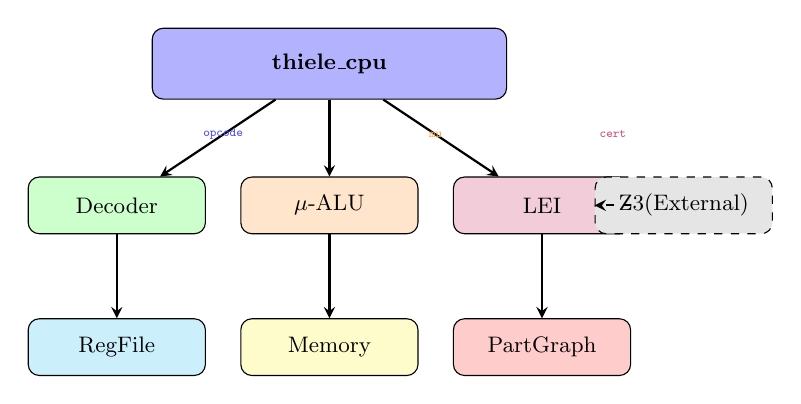
\begin{tikzpicture}[
    module/.style={rectangle, draw, rounded corners, minimum width=2.5cm, minimum height=0.8cm, font=\small},
    arrow/.style={->, thick, >=stealth},
    scale=0.9, transform shape
]
% Top-level CPU
\node[module, fill=blue!30, minimum width=5cm, minimum height=1cm] (cpu) at (0,3) {\textbf{thiele\_cpu}};

% Sub-modules
\node[module, fill=green!20] (decoder) at (-3,1) {Decoder};
\node[module, fill=orange!20] (mualu) at (0,1) {$\mu$-ALU};
\node[module, fill=purple!20] (lei) at (3,1) {LEI};

% Lower components
\node[module, fill=cyan!20] (regfile) at (-3,-1) {RegFile};
\node[module, fill=yellow!20] (memory) at (0,-1) {Memory};
\node[module, fill=red!20] (partgraph) at (3,-1) {PartGraph};

% External interface
\node[module, fill=gray!20, dashed] (z3) at (5,1) {Z3\\(External)};

% Arrows
\draw[arrow] (cpu) -- (decoder);
\draw[arrow] (cpu) -- (mualu);
\draw[arrow] (cpu) -- (lei);
\draw[arrow] (decoder) -- (regfile);
\draw[arrow] (mualu) -- (memory);
\draw[arrow] (lei) -- (partgraph);
\draw[arrow, dashed] (lei) -- (z3);

% Signal annotations
\node[font=\tiny, text=blue!70] at (-1.5,2) {\texttt{opcode}};
\node[font=\tiny, text=orange!70] at (1.5,2) {\texttt{mu}};
\node[font=\tiny, text=purple!70] at (4,2) {\texttt{cert}};
\end{tikzpicture}
\caption{Verilog module hierarchy showing CPU core, $\mu$-ALU, Logic Engine Interface (LEI), and external Z3 connection.}
\label{fig:module-hierarchy}
\end{figure}

\subsection{Module Hierarchy}

The hardware implementation is organized into a CPU core, a $\mu$-accounting unit, a logic-engine interface, and a testbench. The hierarchy mirrors the formal model: the core executes the ISA, the accounting unit enforces $\mu$-monotonicity, and the logic interface brokers certificate checks. This makes the physical design a direct embodiment of the formal step relation.

\subsection{The Main CPU}

\begin{lstlisting}
module thiele_cpu (
    input wire clk,
    input wire rst_n,
    output wire [31:0] cert_addr,
    output wire [31:0] status,
    output wire [31:0] error_code,
    output wire [31:0] partition_ops,
    output wire [31:0] mdl_ops,
    output wire [31:0] info_gain,
    output wire [31:0] mu,  // $\mu$-cost accumulator
    output wire [31:0] mem_addr,
    output wire [31:0] mem_wdata,
    input wire [31:0] mem_rdata,
    output wire mem_we,
    output wire mem_en,
    ...
);
\end{lstlisting}

Key signals:
\begin{itemize}
    \item \textbf{mu}: The $\mu$-accumulator, exported for 3-way isomorphism verification
    \item \textbf{partition\_ops}: Counter for partition operations
    \item \textbf{info\_gain}: Information gain accumulator
    \item \textbf{cert\_addr}: Certificate address CSR
\end{itemize}

% CPU State Machine Diagram
\begin{figure}[ht]
\centering
\begin{tikzpicture}[
    state/.style={circle, draw, minimum size=1.2cm, font=\tiny\bfseries},
    arrow/.style={->, thick, >=stealth, font=\tiny},
    scale=0.85, transform shape
]
% States in a flow
\node[state, fill=blue!20] (fetch) at (0,0) {FETCH};
\node[state, fill=green!20] (decode) at (2.5,0) {DECODE};
\node[state, fill=orange!20] (execute) at (5,0) {EXECUTE};
\node[state, fill=purple!20] (memory) at (7.5,0) {MEMORY};

% Secondary states below
\node[state, fill=yellow!20] (logic) at (2,-2) {LOGIC};
\node[state, fill=cyan!20] (python) at (5,-2) {PYTHON};
\node[state, fill=red!20] (complete) at (8,-2) {COMPLETE};

% ALU wait states
\node[state, fill=gray!20] (aluwait) at (0,-2) {ALU\\WAIT};

% Main flow arrows
\draw[arrow] (fetch) -- (decode);
\draw[arrow] (decode) -- (execute);
\draw[arrow] (execute) -- (memory);
\draw[arrow] (memory) -- (complete);

% Return arrow
\draw[arrow] (complete) to[bend right=40] (fetch);

% Branch arrows
\draw[arrow] (decode) -- (logic) node[midway, left, font=\tiny] {logic op};
\draw[arrow] (decode) -- (python) node[midway, right, font=\tiny] {PYEXEC};
\draw[arrow] (execute) -- (aluwait) node[midway, left, font=\tiny] {ALU};

% Return from branches
\draw[arrow] (logic) -- (complete);
\draw[arrow] (python) -- (complete);
\draw[arrow] (aluwait) to[bend left=30] (execute);

% Title
\node[font=\small\bfseries, above=0.3cm of decode] {12-State FSM};
\end{tikzpicture}
\caption{The CPU finite state machine showing the main execution pipeline and branch states.}
\label{fig:cpu-fsm}
\end{figure}

\subsection{State Machine}

The CPU uses a 12-state FSM:
\begin{lstlisting}
localparam [3:0] STATE_FETCH = 4'h0;
localparam [3:0] STATE_DECODE = 4'h1;
localparam [3:0] STATE_EXECUTE = 4'h2;
localparam [3:0] STATE_MEMORY = 4'h3;
localparam [3:0] STATE_LOGIC = 4'h4;
localparam [3:0] STATE_PYTHON = 4'h5;
localparam [3:0] STATE_COMPLETE = 4'h6;
localparam [3:0] STATE_ALU_WAIT = 4'h7;
localparam [3:0] STATE_ALU_WAIT2 = 4'h8;
localparam [3:0] STATE_RECEIPT_HOLD = 4'h9;
localparam [3:0] STATE_PDISCOVER_LAUNCH2 = 4'hA;
localparam [3:0] STATE_PDISCOVER_ARM2 = 4'hB;
\end{lstlisting}

% Instruction Encoding Diagram
\begin{figure}[ht]
\centering
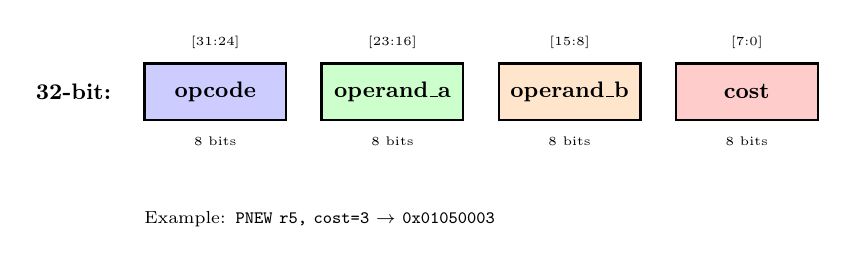
\begin{tikzpicture}[
    bit/.style={rectangle, draw, minimum width=0.4cm, minimum height=0.8cm, font=\tiny},
    field/.style={rectangle, draw, thick, minimum height=0.8cm, font=\small\bfseries},
    scale=0.9, transform shape
]
% 32-bit instruction word
\node[font=\small\bfseries] at (-2,0) {32-bit:};

% Bit fields
\node[field, fill=blue!20, minimum width=2cm] (opcode) at (0,0) {opcode};
\node[field, fill=green!20, minimum width=2cm] (opa) at (2.5,0) {operand\_a};
\node[field, fill=orange!20, minimum width=2cm] (opb) at (5,0) {operand\_b};
\node[field, fill=red!20, minimum width=2cm] (cost) at (7.5,0) {cost};

% Bit positions
\node[font=\tiny] at (0,0.7) {[31:24]};
\node[font=\tiny] at (2.5,0.7) {[23:16]};
\node[font=\tiny] at (5,0.7) {[15:8]};
\node[font=\tiny] at (7.5,0.7) {[7:0]};

% Bit widths below
\node[font=\tiny] at (0,-0.7) {8 bits};
\node[font=\tiny] at (2.5,-0.7) {8 bits};
\node[font=\tiny] at (5,-0.7) {8 bits};
\node[font=\tiny] at (7.5,-0.7) {8 bits};

% Example instruction
\node[font=\scriptsize, text width=8cm, align=left] at (3,-1.8) {
    Example: \texttt{PNEW r5, cost=3} $\rightarrow$ \texttt{0x01050003}
};
\end{tikzpicture}
\caption{Fixed 32-bit instruction encoding ensuring bit-level agreement between hardware and software.}
\label{fig:instruction-encoding}
\end{figure}

\subsection{Instruction Encoding}

Each 32-bit instruction is decoded into opcode and operands. The fixed-width encoding ensures that hardware and software agree on exact bit-level semantics:
\begin{lstlisting}
wire [7:0] opcode = current_instr[31:24];
wire [7:0] operand_a = current_instr[23:16];
wire [7:0] operand_b = current_instr[15:8];
wire [7:0] operand_cost = current_instr[7:0];
\end{lstlisting}

\subsection{$\mu$-Accumulator Updates}

Every instruction atomically updates the $\mu$-accumulator:
\begin{lstlisting}
OPCODE_PNEW: begin
    execute_pnew(operand_a, operand_b);
    // Coq semantics: vm_mu := s.vm_mu + instruction_cost
    mu_accumulator <= mu_accumulator + {24'h0, operand_cost};
    pc_reg <= pc_reg + 4;
    state <= STATE_FETCH;
end
\end{lstlisting}

% μ-ALU Architecture Diagram
\begin{figure}[ht]
\centering
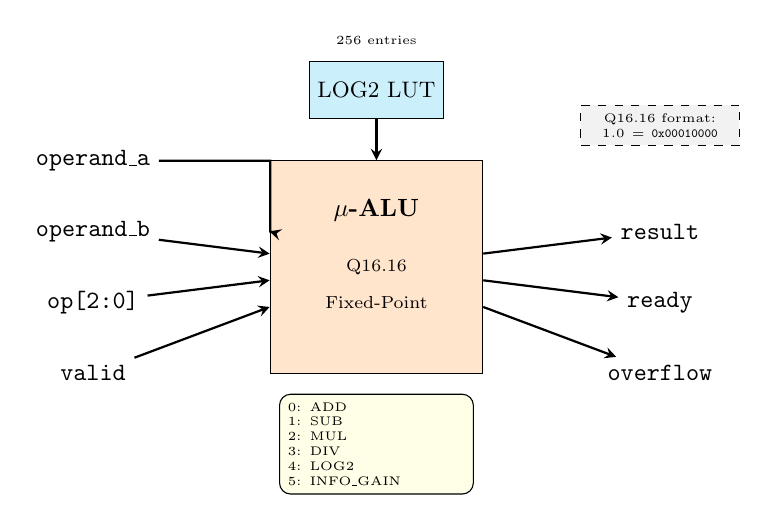
\begin{tikzpicture}[
    block/.style={rectangle, draw, minimum width=2cm, minimum height=0.8cm, font=\small},
    arrow/.style={->, thick, >=stealth},
    scale=0.9, transform shape
]
% Input signals
\node (opa) at (-3,1.5) {\texttt{operand\_a}};
\node (opb) at (-3,0.5) {\texttt{operand\_b}};
\node (op) at (-3,-0.5) {\texttt{op[2:0]}};
\node (valid) at (-3,-1.5) {\texttt{valid}};

% Main ALU block
\node[block, fill=orange!20, minimum width=3cm, minimum height=3cm] (alu) at (1,0) {};
\node[font=\bfseries] at (1,0.8) {$\mu$-ALU};
\node[font=\scriptsize] at (1,0) {Q16.16};
\node[font=\scriptsize] at (1,-0.5) {Fixed-Point};

% Operations list
\node[draw, rounded corners, fill=yellow!10, text width=2.5cm, align=left, font=\tiny] at (1,-2.5) {
    0: ADD\\
    1: SUB\\
    2: MUL\\
    3: DIV\\
    4: LOG2\\
    5: INFO\_GAIN
};

% Output signals
\node (result) at (5,0.5) {\texttt{result}};
\node (ready) at (5,-0.5) {\texttt{ready}};
\node (overflow) at (5,-1.5) {\texttt{overflow}};

% LUT block
\node[block, fill=cyan!20, minimum width=1.5cm] (lut) at (1,2.5) {LOG2 LUT};
\node[font=\tiny] at (1,3.2) {256 entries};

% Arrows
\draw[arrow] (opa) -- (-0.5,1.5) -- (-0.5,0.5) -- (alu);
\draw[arrow] (opb) -- (alu);
\draw[arrow] (op) -- (alu);
\draw[arrow] (valid) -- (alu);
\draw[arrow] (alu) -- (result);
\draw[arrow] (alu) -- (ready);
\draw[arrow] (alu) -- (overflow);
\draw[arrow] (lut) -- (alu);

% Q16.16 annotation
\node[draw, dashed, fill=gray!10, font=\tiny, text width=2cm, align=center] at (5,2) 
    {Q16.16 format:\\$1.0 = \mathtt{0x00010000}$};
\end{tikzpicture}
\caption{The $\mu$-ALU architecture implementing Q16.16 fixed-point arithmetic with LOG2 lookup table.}
\label{fig:mu-alu}
\end{figure}

\subsection{The $\mu$-ALU}

The $\mu$-ALU (\texttt{mu\_alu.v}) implements Q16.16 fixed-point arithmetic:
\begin{lstlisting}
module mu_alu (
    input wire clk,
    input wire rst_n,
    input wire [2:0] op,      // 0=add, 1=sub, 2=mul, 3=div, 4=log2, 5=info_gain
    input wire [31:0] operand_a,
    input wire [31:0] operand_b,
    input wire valid,
    output reg [31:0] result,
    output reg ready,
    output reg overflow
);

localparam Q16_ONE = 32'h00010000;  // 1.0 in Q16.16
\end{lstlisting}

The log2 computation uses a 256-entry LUT for bit-exact results:
\begin{lstlisting}
reg [31:0] log2_lut [0:255];
initial begin
    log2_lut[0] = 32'h00000000;
    log2_lut[1] = 32'h00000170;
    log2_lut[2] = 32'h000002DF;
    ...
end
\end{lstlisting}

\subsection{Logic Engine Interface}

The LEI (\texttt{lei.v}) connects to external Z3:
\begin{lstlisting}
module lei (
    input wire clk,
    input wire rst_n,
    input wire logic_req,
    input wire [31:0] logic_addr,
    output wire logic_ack,
    output wire [31:0] logic_data,
    output wire z3_req,
    output wire [31:0] z3_formula_addr,
    input wire z3_ack,
    input wire [31:0] z3_result,
    input wire z3_sat,
    input wire [31:0] z3_cert_hash,
    ...
);
\end{lstlisting}

\section{Isomorphism Verification}

% Isomorphism Gate Diagram
\begin{figure}[ht]
\centering
\begin{tikzpicture}[
    layer/.style={rectangle, draw, rounded corners, minimum width=2.5cm, minimum height=1cm, font=\small},
    arrow/.style={->, thick, >=stealth},
    compare/.style={diamond, draw, fill=yellow!20, minimum size=1cm, font=\scriptsize},
    scale=0.85, transform shape
]
% Input trace
\node[draw, fill=gray!20, rounded corners] (trace) at (0,0) {Trace $\tau$};

% Three execution paths
\node[layer, fill=blue!20] (coq) at (-3,-2) {Coq\\Extracted};
\node[layer, fill=green!20] (python) at (0,-2) {Python\\VM};
\node[layer, fill=orange!20] (rtl) at (3,-2) {Verilog\\Sim};

% States
\node[draw, rounded corners, fill=blue!10] (scoq) at (-3,-4) {$S_{\text{Coq}}$};
\node[draw, rounded corners, fill=green!10] (spy) at (0,-4) {$S_{\text{Python}}$};
\node[draw, rounded corners, fill=orange!10] (srtl) at (3,-4) {$S_{\text{Verilog}}$};

% Comparison
\node[compare] (cmp) at (0,-5.5) {$=$?};

% Result
\node[draw, thick, fill=green!30, rounded corners] (pass) at (0,-7) {\textbf{PASS}};

% Arrows
\draw[arrow] (trace) -- (coq);
\draw[arrow] (trace) -- (python);
\draw[arrow] (trace) -- (rtl);

\draw[arrow] (coq) -- (scoq);
\draw[arrow] (python) -- (spy);
\draw[arrow] (rtl) -- (srtl);

\draw[arrow] (scoq) -- (cmp);
\draw[arrow] (spy) -- (cmp);
\draw[arrow] (srtl) -- (cmp);

\draw[arrow] (cmp) -- (pass);

% Annotations
\node[font=\scriptsize, text width=2cm, align=center] at (-4.5,-2) {JSON\\snapshot};
\node[font=\scriptsize, text width=2cm, align=center] at (4.5,-2) {VCD\\waveform};
\end{tikzpicture}
\caption{The 3-way isomorphism gate: instruction trace $\tau$ is executed on all three layers, and state projections must match exactly.}
\label{fig:isomorphism-gate}
\end{figure}

\subsection{The Isomorphism Gate}

The 3-way isomorphism is verified by a test that:
\begin{enumerate}
    \item Generate instruction trace $\tau$
    \item Execute $\tau$ on Python VM $\rightarrow$ state $S_{\text{py}}$
    \item Execute $\tau$ on extracted runner $\rightarrow$ state $S_{\text{coq}}$
    \item Execute $\tau$ on Verilog sim $\rightarrow$ state $S_{\text{rtl}}$
    \item Assert $S_{\text{py}} = S_{\text{coq}} = S_{\text{rtl}}$
\end{enumerate}

\subsection{State Projection}

For comparison, states are projected to canonical summaries tailored to the gate being exercised. The extracted runner emits a full JSON snapshot (pc, $\mu$, err, regs, mem, CSRs, graph), which can be projected down to subsets. The compute gate uses only registers and memory, while the partition gate uses canonicalized module regions. A full projection helper is therefore a \emph{superset} view, not the only comparison performed:
\begin{lstlisting}
def project_state_full(state):
    return {
        "pc": state.pc,
        "mu": state.mu,
        "err": state.err,
        "regs": list(state.regs[:32]),
        "mem": list(state.mem[:256]),
        "csrs": state.csrs.to_dict(),
        "graph": state.graph.to_canonical(),
    }
\end{lstlisting}

% Inquisitor Workflow Diagram
\begin{figure}[ht]
\centering
\begin{tikzpicture}[
    stage/.style={rectangle, draw, rounded corners, minimum width=2.5cm, minimum height=1cm, font=\small},
    check/.style={diamond, draw, fill=yellow!20, minimum size=0.8cm, font=\tiny},
    arrow/.style={->, thick, >=stealth},
    scale=0.85, transform shape
]
% Stages
\node[stage, fill=blue!20] (scan) at (0,0) {Scan\\Sources};
\node[stage, fill=green!20] (build) at (3,0) {Build\\Proofs};
\node[stage, fill=orange!20] (iso) at (6,0) {Run\\Isomorphism};
\node[stage, fill=purple!20] (report) at (9,0) {Generate\\Report};

% Checks
\node[check] (c1) at (1.5,0) {};
\node[check] (c2) at (4.5,0) {};
\node[check] (c3) at (7.5,0) {};

% Arrows
\draw[arrow] (scan) -- (c1);
\draw[arrow] (c1) -- (build);
\draw[arrow] (build) -- (c2);
\draw[arrow] (c2) -- (iso);
\draw[arrow] (iso) -- (c3);
\draw[arrow] (c3) -- (report);

% What each stage checks
\node[font=\tiny, text width=2cm, align=center, below=0.3cm of scan] {No \texttt{Admitted}\\No \texttt{admit.}\\No \texttt{Axiom}};
\node[font=\tiny, text width=2cm, align=center, below=0.3cm of build] {206 proofs\\compile\\successfully};
\node[font=\tiny, text width=2cm, align=center, below=0.3cm of iso] {3-way\\state match};
\node[font=\tiny, text width=2cm, align=center, below=0.3cm of report] {HIGH: 0\\MEDIUM: 2\\LOW: 4};

% Pass/Fail output
\node[draw, thick, fill=green!30, rounded corners] (pass) at (12,0) {\textbf{CI PASS}};
\draw[arrow] (report) -- (pass);

% Ultra-strict annotation
\node[draw, dashed, fill=red!10, font=\tiny, text width=3cm, align=center] at (3,-2.5) 
    {\texttt{--ultra-strict}:\\Fails on MEDIUM\\in kernel files};
\end{tikzpicture}
\caption{The Inquisitor verification workflow: source scanning, proof building, isomorphism testing, and report generation.}
\label{fig:inquisitor-workflow}
\end{figure}

\subsection{The Inquisitor}

The Inquisitor enforces the verification rules:
\begin{itemize}
    \item Scans the proof sources for \texttt{Admitted}, \texttt{admit.}, \texttt{Axiom}
    \item Verifies that the proof build completes successfully
    \item Runs isomorphism gates
    \item Reports HIGH/MEDIUM/LOW findings
\end{itemize}

The repository must have 0 HIGH findings to pass CI.

\section{Synthesis Results}

\subsection{FPGA Targeting}

The RTL can be synthesized for Xilinx 7-series FPGAs:
\begin{lstlisting}
$ yosys -p "read_verilog thiele_cpu.v; synth_xilinx -top thiele_cpu"
\end{lstlisting}

\subsection{Resource Utilization}

Under a reduced configuration (fewer modules, smaller regions):
\begin{itemize}
    \item NUM\_MODULES = 4
    \item REGION\_SIZE = 16
    \item Estimated LUTs: $\sim$2,500
    \item Estimated FFs: $\sim$1,200
\end{itemize}

Full configuration:
\begin{itemize}
    \item NUM\_MODULES = 64
    \item REGION\_SIZE = 1024
    \item Estimated LUTs: $\sim$45,000
    \item Estimated FFs: $\sim$35,000
\end{itemize}

\section{Toolchain}

\subsection{Verified Versions}

\begin{itemize}
    \item Coq 8.18.x (OCaml 4.14.x)
    \item Python 3.12.x
    \item Icarus Verilog 12.x
    \item Yosys 0.33+
\end{itemize}

\subsection{Build Commands}

\begin{lstlisting}
# Example commands (paths may vary by environment):
# - build the Coq kernel
# - run the two isomorphism tests
# - simulate the RTL testbench
# - run full synthesis when toolchains are installed
\end{lstlisting}

% Chapter 4 Summary Diagram
\begin{figure}[ht]
\centering
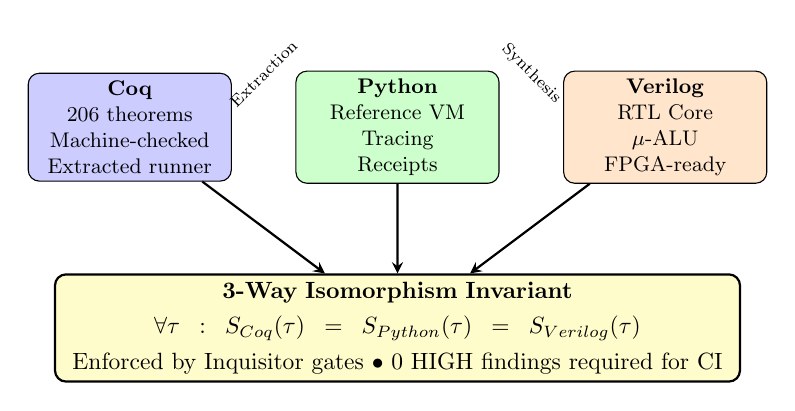
\begin{tikzpicture}[
    box/.style={rectangle, draw, rounded corners, minimum width=3cm, minimum height=1.5cm, font=\small, text width=2.8cm, align=center},
    arrow/.style={->, thick, >=stealth},
    scale=0.85, transform shape
]
% Three layers as boxes
\node[box, fill=blue!20] (coq) at (-4,0) {\textbf{Coq}\\206 theorems\\Machine-checked\\Extracted runner};
\node[box, fill=green!20] (python) at (0,0) {\textbf{Python}\\Reference VM\\Tracing\\Receipts};
\node[box, fill=orange!20] (verilog) at (4,0) {\textbf{Verilog}\\RTL Core\\$\mu$-ALU\\FPGA-ready};

% Central invariant at bottom
\node[draw, thick, fill=yellow!20, rounded corners, text width=10cm, align=center] (inv) at (0,-3) 
    {\textbf{3-Way Isomorphism Invariant}\\[3pt]
     $\forall \tau: S_{\text{Coq}}(\tau) = S_{\text{Python}}(\tau) = S_{\text{Verilog}}(\tau)$\\[3pt]
     Enforced by Inquisitor gates $\bullet$ 0 HIGH findings required for CI};

% Arrows to invariant
\draw[arrow] (coq) -- (inv);
\draw[arrow] (python) -- (inv);
\draw[arrow] (verilog) -- (inv);

% What flows between layers
\node[font=\scriptsize, rotate=45] at (-2,0.8) {Extraction};
\node[font=\scriptsize, rotate=-45] at (2,0.8) {Synthesis};
\end{tikzpicture}
\caption{Chapter 4 summary: Three implementation layers bound by the central isomorphism invariant, enforced through automated verification gates.}
\label{fig:ch4-summary}
\end{figure}

\section{Summary}

The 3-layer implementation ensures:
\begin{itemize}
    \item \textbf{Logical Certainty}: Coq proofs guarantee properties hold for all inputs
    \item \textbf{Operational Visibility}: Python traces expose every state transition
    \item \textbf{Physical Realizability}: Verilog synthesizes to real hardware
\end{itemize}

The binding across layers is not aspirational—it is enforced through automated isomorphism gates. The Inquisitor ensures that no admits, no axioms, and no semantic divergences are ever committed to the main branch.
